\section{Concurrency}\label{sec:concurrency}
The term concurrency is a general term for ways a computer system performs multiple tasks 'at the same time'. It covers the \textit{simulation} of multiple tasks running at the same time through process switching, as well as work done in parallel. To disambiguate, based on the definition:

\blockcquote{Bryant2016}{We use the term concurrency to refer to the general concept of a system with multiple, simultaneous activities, and the term parallelism to refer to the use of concurrency to make a system run faster.}

We infer that parallelism is a type of concurrency with the purpose to speed up the system, while concurrency in general may have purposes not related to speed.

Concurrency is a large and hardware dependant subject. To prevent falling into a concurrency rabbit hole, the limitations of the Arduino hardware in relation to concurrency, specifically the \gls{cpu}, is explored before concurrency in general. This is done because the project is, first and foremost, about programming language design - not concurrency.

\subsection{Arduino hardware}\label{subsec:arduinohardware}
The Arduino Uno board uses the ATmega328P microcontroller \cite{ArduinoUno}. The architecture of this microcontroller is a scalar single core processor, without hyperthreading(intel) or \gls{smt} (AMD) equivalents \cite{ATmega328P}.

Since there is only a single core, and that core does not contain any duplicate copies of CPU hardware (for multithreading), the only hardware parallelism on the Arduino Uno is instruction-level parallelism, and only to the level of up to 1 instruction per clock cycle (scalar). This is also handled directly by the \gls{cpu}, and does not impact the instruction set available to developers.


\begin{figure}[htb!]
    \centering
    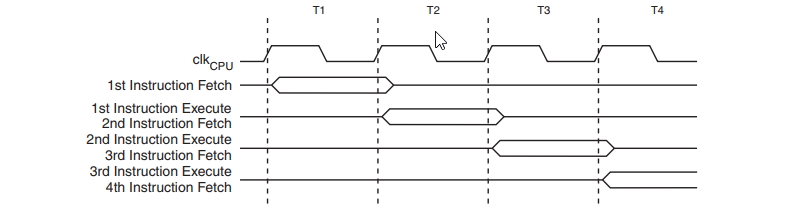
\includegraphics[width=\textwidth]{figures/Arduino_Pipeline.png}
    \caption{The parallel intruction fetches and intruction executions \cite{ATmega328P}}
    \label{fig:arduinopipeline}
\end{figure}


The Arduino is therefore a uniprocessor\cite{Bryant2016} - its architecture does not support parallel processing - and for the remainder of the report the term concurrency refers to concurrency \textbf{without parallelism}.

\subsection{Models of concurrency}\label{subsec:modelsofcon}
Even unicore processors can support several models for concurrency at the application software level. This makes sense since a computer often has more processes running than it has \glspl{cpu}. This is done through interweaving instructions of different processes, which lets the \gls{cpu} appear to run multiple programs.

This interweaving is commonly handled through an \gls{os}, which manages the hardware resources \cite{Bryant2016}. A few different approaches for interweaving processes are supported by the \gls{os}:

\subsubsection{Processes}
In this model the kernel, the portion of the \gls{os} code that resides in memory while the system is running, schedules and maintains each logical control flow, called a process. Each process has its own 

\blockcquote{Bryant2016}{The kernel is the portion of the operating system code that is always resident in memory.}


\subsubsection{I/O multiplexing}


\subsubsection{Threads}



% Note: Operating systems, libraries, scheduling, and differences between the options.




\section*{deprecated for now}
The scheduler is usually what takes care of these choices and prioritization

Concurrency is used for things like coordinating the execution of processes to maximize throughput. Concurrency is not to be confused with parallelism, which requires multiple cores because you have to do several things at the same time. Concurrency, on the other hand, does not need to be at the same time, just in the right order at the correct times, so it is possible to do with a single core. Since the Arduino has only a single core, this project deals with concurrency without parallelism.

It is possible to achieve concurrency on Arduino, but not without scheduling of some kind. Scheduling is to schedule different tasks to run on the same CPU, fooling users to think that they all run at the same time, while in fact it is running different tasks very fast and switching between them. This scheduling is not built into Arduino so the project will have to decide on how to achieve it. Part of the problem is choosing how to do this, while also keeping the end-user in mind. A hobbyist typically tries to achieve concurrency through the standard functions in Arduino, but many of these functions are not ideal for concurrency.

Several tutorials on how to implement different techniques to achieve some sort of concurrency in Arduino exist. These techniques include Milis() and Interrupt(). Milis() uses the milis function to tell the time, while not pausing to achieve the ability to wait and not do unnecessary tasks at all times. The interrupt() function, on the other hand, cancels the process if something happens, and this can be used to change between different tasks.

\todo[inline]{Maybe include references or examples?}
